\documentclass[a4paper, 14pt]{extarticle}
\title{	Анализ платежного баланса Российской Федерации с помощью модели внешнеэкономической деятельности}
%%% Работа с русским языком
% правильно: fontspec + polyglossia 
% не надо загружать mathtext, и без него русский в формулах читается,
% зато он конфликтует с polyglossia

% не надо etex
% только newcommand вместо def


%%% Дополнительная работа с математикой
\usepackage{amsfonts,amssymb,amsthm,mathtools} % AMS
\usepackage{amsmath}
\usepackage{icomma} % "Умная" запятая: $0,2$ --- число, $0, 2$ --- перечисление


% https://tex.stackexchange.com/questions/73684
% решаем конфликт amssymb vs dingbat за checkmark
\usepackage{savesym}
\savesymbol{checkmark}
\usepackage{dingbat}
\usepackage{epigraph}

\usepackage{caption}
\usepackage{geometry} 
\geometry{left=2cm}
\geometry{right=2cm}
\geometry{top=2cm}
\geometry{bottom=2cm}
% \usepackage[misc,clock, weather, alpine]{ifsym}

\usepackage{graphicx}

%% Шрифты
% \usepackage{euscript}	 % Шрифт Евклид
% \usepackage{mathrsfs} % Красивый матшрифт



%%% Работа с картинками
\setlength\fboxsep{3pt} % Отступ рамки \fbox{} от рисунка
\setlength\fboxrule{1pt} % Толщина линий рамки \fbox{}
\usepackage{wrapfig} % Обтекание рисунков и таблиц текстом

%%% Работа с таблицами
\usepackage{array,tabularx,tabulary,booktabs} % Дополнительная работа с таблицами
\usepackage{longtable}  % Длинные таблицы
\usepackage{multirow} % Слияние строк в таблице
% \usepackage{upgreek}

% \usepackage{enumerate}
\usepackage{dsfont}
\usepackage{todonotes}




%%% Гиперссылки

\usepackage{xcolor}
\usepackage{hyperref}
\definecolor{linkcolor}{HTML}{6b039b} % цвет ссылок
\definecolor{urlcolor}{HTML}{6b039b} % цвет гиперссылок
\definecolor{citecol}{HTML}{8a2be2} % ссылки на литру


\hypersetup{pdfstartview=FitH,  linkcolor=linkcolor,urlcolor=urlcolor, citecolor=citecol, colorlinks=true}

%%% Заголовок
\usepackage{fancyhdr}
\setlength{\headheight}{10.2pt}
\pagestyle{fancyplain}

%\usepackage{minted}

\usepackage{fontspec} 

% Ligatures=TeX is on by default
% https://tex.stackexchange.com/questions/323542/
\setmainfont{Times New Roman}
\newfontfamily{\cyrillicfonttt}{Times New Roman}

\usepackage{polyglossia} % для выбора языка в xelatex

\setmainlanguage{russian}
\setotherlanguages{english}

\usepackage{csquotes}

\usepackage{verbatim}
\usepackage{comment}


%\graphicspath{{images/}{../images/}}
%\usepackage{subfiles}

%\usepackage[backend=biber,bibencoding=utf8,sorting=nty,maxcitenames=4,style=numeric-verb]{biblatex}
\usepackage[bibencoding = utf8,
backend = biber,
sorting = nty,
style=numeric-verb]{biblatex}

\addbibresource{document.bib}


\linespread{1.5}



%% эконометрические сокращения
\DeclareMathOperator{\sVar}{sVar}
\DeclareMathOperator{\sCov}{sCov}
\DeclareMathOperator{\sCorr}{sCorr}
\DeclareMathOperator{\cov}{Cov}
\DeclareMathOperator{\Var}{Var}
\DeclareMathOperator{\Cov}{Cov}
\DeclareMathOperator{\Corr}{Corr}

\DeclareMathOperator{\sgn}{sgn}
\DeclareMathOperator*{\argmin}{arg\,min}
\DeclareMathOperator*{\argmax}{arg\,max}
\DeclareMathOperator*{\amn}{arg\,min}
\DeclareMathOperator*{\amx}{arg\,max}
\DeclareMathOperator{\tr}{tr}
\DeclareMathOperator*{\plim}{plim}

%% лаг
\renewcommand{\L}{\mathrm{L}}
\newcommand \mL{\mathcal{L}}
\newcommand{\lsum}{\sum\limits}


\renewcommand{\labelitemiii}{$\textcolor{violet}{\diamond}$}

\usepackage[inline,shortlabels]{enumitem}

\usepackage{url}

\setlength{\parskip}{0.5em}
%\setlength{\parindent}{0cm}


\begin{document}
\begin{center}
	{\textbf{Анализ платежного баланса Российской Федерации с помощью модели внешнеэкономической деятельности
	}}
\end{center}

{\bf Конкурс:} магистратура.

{\bf Ключевые слова:} внешнеэкономическая деятельность, платежный баланс, валютный курс, бюджетное правило.

\begin{abstract}
	В работе построена модель внешнеэкономической деятельности Российской Федерации, включающая системы уравнений для счета текущих операций и его компонент, финансового счета, валютного курса, объема покупки валюты Министерством финансов в рамках бюджетного правила, а также ряда показателей топливных рынков. Модель предназначена для построения сценарных прогнозов основных показателей внешнеэкономической деятельности РФ на краткосрочный период при различных траекториях экзогенных переменных, в частности цен на нефть, темпа роста ВВП и ключевой ставки. В работе рассмотрены три сценария на $2020$ год и на основании прогнозов модели сделаны выводы об устойчивости платежного баланса страны в ответ на различные экзогенные шоки.
\end{abstract}

{\bf Тематическое направление:} математическая экономика.

{\bf Классификатор JEL:} C51, C53.

\newpage
\section{Введение}
Платежный баланс Российской Федерации является важным источником статистических данных о внешнеэкономической деятельности государства. 
В нем отражены экономические операции между резидентами и нерезидентами страны за определенный период времени. 
Платежный баланс охватывает экономическую деятельность центрального банка, банков, органов государственного управления, домашних хозяйств, других финансовых и нефинансовых учреждений.

Основными агрегатами платежного баланса РФ являются счет текущих операций, счет операций с капиталом и финансовый счет. 
Счет текущих операций отражает потоки товаров, услуг, первичных и вторичных доходов между резидентами и нерезидентами страны.  
Счет операций с капиталом включает операции с непроизведенными нефинансовыми активами и международными трансфертами. 
В финансовом счете отражается приобретение резидентами иностранных финансовых активов  и принятие ими финансовых обязательств по отношению к нерезидентам.
Отдельно выделяется статья «Чистые ошибки и пропуски».
Она необходима для балансирования возможных статистических расхождений, которых по определению «двойной записи» быть не должно, но которые неизбежно возникают из-за использования разного набора источников для отражения транзакций в платежном балансе.

Сальдо платежного баланса является одним из ключевых показателей внешнеэкономического положения страны. 
Особый интерес представляет динамика отдельных его компонент .
В частности, для России, как экспортно - ориентированной экономики с высокой (около $60 \%$) долей топливных ресурсов в экспорте, показательным является торговый баланс, который в значительной степени формирует счет текущих операций. 
По этой причине счет текущих операций оказывается очень чувствительным к колебаниям на мировых рынках, в частности динамика счета тесно связана не только с ценами на нефть и объемами ее  экспорта, но и с курсом рубля по отношению к другим валютам, особенно к доллару.

В самых общих словах механизм взаимосвязи платежного баланса и валютного курса можно описать следующим образом. 
Отток капитала из страны либо резкое снижение сальдо внешней торговли, вызванное, например, падением нефтяных доходов либо снижением экспорта из-за введения санкций, если они не скомпенсированы друг другом, как правило, ведут к ослаблению курса рубля. 
В связи с этим велика заинтересованность монетарных властей и других лиц, принимающих решения, в надежном прогнозе различных компонент платежного баланса.
Особенно востребованной кажется возможность построения сценарных прогнозов, которые бы позволяли учесть в модели мнения экспертов и различные варианты реализации внешней и внутренней политики, рассматривать эффекты возможных шоков и их влияние на устойчивость платежного баланса.

Комплексной модели, описывающей взаимозависимости переменных платежного баланса Российской Федерации между собой и с другими макроэкономическими и финансовыми показателями, на данный момент нет.  

Целью данной работы является построение, описание и программная реализация модели внешнеэкономической деятельности РФ, основной частью и предназначением которой является возможность прогнозирования основных агрегатов платежного баланса и их компонент на краткосрочный (до года) и среднесрочный (до трех лет) периоды в месячном измерении. 
Важной особенностью модели является возможность восстанавливать отсутствующие месячные данные, используя квартальные значения. 
В модели также осуществляется прогноз валютного курса, покупки валюты Минфином, а также ряда показателей экспорта нефти, газа и нефтепродуктов.

Далее работа будет устроена следующим образом. 
В первой главе изложен обзор литературы, в котором освещены различные способы моделирования внешнеэкономической деятельности и платежного баланса. 
Во второй главе представлен обзор данных по российской внешнеэкономической деятельности, используемых в исследовании, описана модель прогнозирования платежного баланса Российской Федерации и приведено сравнение ее прогнозной силы с более простыми моделями (ARIMA, ets, сезонная наивная модель).
В третьей главе рассмотрено несколько сценариев динамики экзогенных переменных, выступающих в модели в качестве предикторов. 
Для каждого из сценариев построены прогнозы основных агрегатов и компонент платежного баланса, а также некоторых других переменных, характеризующих внешнеэкономическую деятельность РФ.
\newpage
\section{Основная часть}
\subsection{Обзор литературы}
Существует большое количество подходов к моделированию внешнеэкономической деятельности. 
При этом редко встречаются работы, в которых платежный баланс включается в модели в виде системы в разбивке на его отдельные компоненты.
Тем не менее предшествующие исследования предлагают ценные гипотезы о зависимости различных переменных, характеризующих внешнеэкономическую деятельность. 

Одной из основополагающих является работа Robert. A Mundell (1963) \autocite{mundell1963capital}, в которой рассматривается малая открытая экономика с совершенной мобильностью капитала.
Автор изучает разные последствия фискальной и монетарной политики в зависимости от существующего режима валютного курса: плавающего или фиксированного.
В частности, он приходит к выводу, что без значительного влияния на уровень выпуска и безработицы при фиксированном валютном курсе оказывать влияние на динамику резервов можно через каналы монетарной политики. 
При плавающем валютном курсе, не нарушая равновесия на других рынках, остается возможность регулировать торговый баланс только методами фискальной политики.

Важной частью исследованиий Mundell (1960) \autocite{mundell1960monetary} являлся динамический анализ кризисов платежного баланса, ключевые достижения в котором позднее были сделаны в моделях, предложенных Krugman (1979) \autocite{krugman1979model} и Obstfeld (1986) \autocite{obstfeld1986speculative}. 
Под кризисом платежного баланса в этих работах следует понимать ситуации, когда резервы Центрального Банка опускаются ниже некоторого критического уровня и повышается угроза обесценения валютного курса.

Позднее, с усилением процессов международной мобильности капитала и экономической интеграции, идеи Mundell, в том числе в части изучения механизмов платежного баланса, были пересмотрены уже в рамках современной  международной макроэкономики в работе Mendoza E., Uribe M. (1999) \autocite{mendoza1999business}. 
Авторами была представлена модель двухсекторной малой открытой экономики, в которой фирмы производят торгуемые и неторгуемые товары с помощью двух факторов производства: капитала и рабочей силы. 
Фирмы и домохозяйства имееют неограниченный доступ к международному рынку капитала с совершенной конкуренцией, агенты имеют рациональные ожидания. 
Авторы строят межвременную модель общего равновесия, в которой вероятность обесценения валютного курса является эндогенной переменной и зависит от изменения величины иностранных резервов и величины дефицита платежного баланса.  
В работе сделано важное замечание о причинах кризисов платежного баланса.
Основным тригером, по мнению авторов, является отсутствие доверия частного сектора, которое неявным образом заданно с помощью функции реакции политики центрального банка. 
Данная функция устанавливает отрицательную зависимость между вероятностью обесценения национальной валюты и объемом иностранных резервов. 
Модель позволяет анализировать влияние устойчивости фискальной политики государства и  спекулятивных атак на вероятность возникновения кризиса.

С начала 1990-х годов происходил активный процесс перехода многих стран к режиму инфляционного таргетирования. 
В связи с этим получили развитие модели, анализирующие влияние различных режимов монетарной политики на кризис платежного баланса.  
В работе Kumhof $\&$ Yan (2007) \autocite{kumhof2007balance} построена модель малой открытой экономики с режимом таргетирования инфляции.
В ее рамках изучается степень влияния спекулятивных атак на платежный баланс в зависимости от сложности выполнения центральным банком взятых на себя обязательств: наиболее болезненное влияние спекулятивные атаки оказывают на экономику с таргетируемым обменным курсом; наименьшее — на экономику, придерживающуюся таргетирования индекса потребительских цен, внутренней инфляции или денежной базы. 
В работе авторы строят микрообоснованную модель кризисов первого поколения, изначально предложенную в статье Calvo (1987) \autocite{calvo1987balance}.

Модель малой открытой экономики с режимом таргетирования инфляции была также предложена в работе \autocite{mansoorian2006employment}.
В дополнение к предшествующим исследованиям в этой модели авторы рассматривают ограничение «деньги вперед» (cash-in-advance). 
В работе исследуется влияние роста уровня инфляции на безработицу, инвестиции, потребление и счет текущих операций. 
Авторы отмечают, что рост инфляции сопровождается положительным сальдо счета текущих операций, так как падение выпуска вследствие снижения занятости уравновешивается падением потребления и инвестиций.

В последние годы высокую популярность имеют динамические стохастические модели общего равновесия (DSGE) с уравнением на платежный баланс.
Их преимуществом является высокая гибкость при моделировании поведения экономических агентов, например, Центрального банка и монетарных властей.
Другим существенным плюсом является возможность проводить эмпирический анализ, калибруя модель для изучения и прогнозирования экономики отдельной страны. 
В рамках DSGE-подхода после этапа решения модели, происходит симуляция экономики и строятся функции импульсного отклика эндогенных переменных в ответ на экзогенные шоки.

В статье Escudé’s (2013) \autocite{escude2013dsge} авторы строят DSGE модель, в которой с помощью функции потерь специального вида моделируют различные типы интервенций монетарных властей: интервенции только на валютный рынок, только на рынок облигаций и одновременно на два рынка. 
Наряду с другими уравнениями, система включает уравнение на экспорт, счет текущих операций и сальдо торгового баланса. 
Оценка параметров модели показала, что Центральный банк несет меньшие потери, если использует оба типа интервенций. 
Такой режим дает монетарным властям возможность влиять на потоки частных капиталовложений путем достижения определенного уровня премии за риск.

В статье Cubas, G. (2011) \autocite{cubas2011dynamic} DSGE модель внешнеэкономической деятельности построена и откалибрована для экономики Уругвая. 
В работе предлагается методология для анализа влияния трансмиссии монетарной политики на основные макроэкономические индикаторы, в том числе на сальдо платежного баланса, заданного с помощью динамического уравнения. 
Наряду с ним в системе рассматривается набор взаимосвязанных макропеременных, таких как премия за риск, инфляция, размер интервенций Центрального банка, средняя цена экспорта товаров и услуг.

На практике для моделирования отдельных компонент платежного баланса нередко используются более простые статистические модели.
Их преимущество в простоте вычисления и отсутствии необходимости жестких теоретических предпосылок о взаимосвязи переменных и поведении агентов.
В статье Freund (2005) \autocite{freund2005current} анализируются различные детерминанты процесса корректировки (перехода от дефицита к профициту) платежного баланса в индустриальных странах. 
В качестве тестируемых моделей используется набор простых линейных регрессий.
В работе изучается только динамика счета текущих операций, так как обычно именно он составляет наибольшую часть платежного баланса развитых стран. 
Кроме того, торговый баланс, входящий в счет текущих операций, как правило, является основным драйвером дефицита платежного баланса.
Автор показывает, что замедление темпов роста ВВП и реальное удорожание валюты являются главными триггерами изменения долгосрочной динамики счета текущих операций.  

В другой работе Kandil $\&$ Greene (2002) \autocite{kandil2002impact} показали, что ключевые агрегаты платежного баланса (счет текущих операций и финансовый счет) чувствительны к циклическим факторам в экономике. 
Авторы обнаружили наличие коинтеграции между счетами платежного баланса и темпом прироста реального ВВП, с одной стороны, и реальным эффективным обменным курсом, с другой. Модель оценивалась в два шага. 
Сначала был проведен анализ на коинтеграцию, который позволяет уловить долгосрочные взаимосвязи между компонентами платежного баланса и циклическими макропеременными. 
Затем авторы оценили набор уравнений в приведенной форме для сальдо счета текущих операций, финансового счета и его компонет. 
Модели оценивались как на квартальных, так и на месячных данных. 
Мотивация такого подхода заключалась в том что использование данных с разной частотностью позволит уловить взаимозависимости переменных в среднесрочном периоде и одновременно учесть влияние циклических факторов, которое лучше заметно в краткосрочном периоде.

Позднее Akbas, Later, Senturk, $\&$ Sancar  (2013) \autocite{akbas2013testing} продемонстрировали
 связь между дефицитом счета текущих операций и размером иностранных прямых инвестиций.

Модель внешнеэкономической деятельности экономики России построена в работе Пильник $\&$ Ужегов.
Она представляет собой набор систем уравнений, описывающих основные компоненты платежного баланса РФ, а также ряд других переменных внешнеэкономической деятельности.
С ее помощью можно осуществлять прогноз основных агрегатов платежного баланса на краткосрочный (до года) и среднесрочный (до трех лет) периоды.
Динамика переменных платежного баланса объясняется с помощью ряда экзогенных макроэкономических и финансовых показателей, а также с помощью эндогенных переменных. 
Оценка модели происходит на месячных и квартальных данных.


\newpage
\subsection{Модель}
\epigraph{Вы берете часы, какие угодно, хоть стенные, хоть башенные, можно даже игрушечные, все равно. Лишь бы у них были стрелки и циферблаты. Конечно, в течение большей части суток пользоваться таким хронометром не придется ... зато два раза в сутки ваш хронометр совершенно точно покажет время}{\textit{Капитан Врунгель}}
Модель, описанная в данной работе, развивает исследовательский вопрос, поднятый в статье Пильник $\&$ Ужегов \autocite{пильник2017модель}. 
Она представляет собой набор балансовых и эконометрических соотношений, сгруппированных в системы либо оцениваемых независимо. 
Балансовые соотношения должны быть выполнены по определению той или иной компоненты платежного баланса. 
Например, совокупный экспорт за месяц равен сумме экспорта товаров и услуг за тот же период.
Эконометрические соотношения устанавливают статистическую взаимосвязь между эндогенными и экзогенными переменными в модели и оцениваются с помощью минимизации целевой функции специального вида.

\subsubsection{Переменные}

Все переменные можно разделить на экзогенные, заданные извне и не объясняемые моделью, и эндогенные, динамика которых моделируется при решении системы.

Модель внешнеэкономической деятельности состоит из нескольких блоков.
Уравнения первого блока описывают динамику различных компонент платежного баланса. 
Второй блок посвящен моделированию экспорта основных топливных ресурсов, формирующих, как было показано в разделе \hyperref[sub:data]{Данные}, большую часть экспорта России, а именно нефти, нефтепродуктов и природного газа.
Также в модели предусмотрены отдельные уравнения на валютный курс и на размер покупки валюты Министерством финансов в рамках бюджетного правила.
Моделирование платежного баланса, переменных топливных рынков, валютного курса и покупки валюты в рамках одной большой модели внешнеэкономической деятельности обусловлено схожим набором экзогенных показателей, которые предположительно помогают объяснить динамику этих переменных и строить надежные прогнозы на краткосрочный и среднесрочный периоды.

Для удобства ниже приведен список эндогенных моделируемых переменных. 
В таблице \ref{tab:1} представлены переменные блока платежного баланса, а также их обозначения, используемые в скрипте, написанном для оценки модели на языке программирования R.
Переменные разделены на две группы: те, для которых оцениваются коэффициенты в эконометрических соотношениях, и балансовые переменные, значения которых получаются из балансовых соотношений.

В таблице \ref{tab:2} перечислены обозначения эндогенных переменных, оцениваемых в других блоках модели.

В таблице \ref{tab:3} перечислены используемые в модели экзогенные переменные и их обозначения.


\begin{center}
	\small
	\begin{tabular}{ l | c }
		\toprule
		Эндогенные переменные  & Обозначение в модели  \\
		\midrule
		\multicolumn{2}{c}{Эконометрические соотношения}\\
		\midrule 
		экспорт прочих товаров & \textit{ r\_exp\_othg } \\
		экспорт услуг & \textit{ r\_exp\_serv } \\
		импорт товаров &  \textit{ r\_imp\_goods } \\  
		импорт услуг &  \textit{ r\_imp\_serv } \\  
		баланс оплаты труда &  \textit{ r\_bal\_wage } \\  
		баланс ренты и вторичных доходов &  \textit{ r\_bal\_rent\_sinc } \\ 
		баланс инвестиционных доходов &  \textit{ r\_bal\_inv } \\
		изменение резервных активов &  \textit{ dif\_reserves } \\
		чистые ошибки и пропуски &  \textit{ r\_errors } \\
		\midrule
		\multicolumn{2}{c}{Балансовые соотношения}\\
		\midrule
		экспорт товаров & \textit{ r\_exp\_goods } \\
		импорт  &  \textit{ r\_imp\_all } \\  
		экспорт  &  \textit{ r\_exp\_all } \\  
		торговый баланс  &  \textit{ r\_bal\_trade } \\
		баланс услуг  &  \textit{ r\_bal\_serv } \\
		счет текущих операций  &  \textit{ r\_cur\_account } \\
		финансовый баланс  &  \textit{ r\_bal\_fin } \\
		\bottomrule
	\end{tabular}
\normalsize
\captionof{table}{Модель платежного баланса}\label{tab:1}
\end{center}



	\begin{center}
		\small
		\begin{tabular}{ l | c }
			\toprule
			  Эндогенные переменные  &  Обозначение в модели  \\
			\midrule
			\multicolumn{2}{c}{модель нефти}\\
			\midrule
			 средняя цена экспорта нефти & \textit{ p\_exp\_oil } \\ 
			 объем экспорта нефти & \textit{ v\_exp\_oil } \\
			выручка от экспорта нефти &  \textit{ r\_exp\_oil } \\ 
			\midrule
			\multicolumn{2}{c}{модель нефтепродуктов} \\
			\midrule
			средняя цена экспорта нефтепродуктов & \textit{ p\_exp\_op } \\ 
			объем экспорта нефтепродуктов & \textit{ v\_exp\_op } \\
			выручка от экспорта нефтепродуктов &  \textit{ r\_exp\_op } \\ 
			\midrule
			\multicolumn{2}{c}{модель газа}\\
			\midrule
			средняя цена экспорта газа & \textit{ p\_exp\_gas } \\ 
			объем экспорта газа & \textit{ v\_exp\_gas } \\
			выручка от экспорта газа &  \textit{ r\_exp\_gas } \\ 
			\midrule
			валютный курс (USD/RUB) & \textit{ rub\_usd } \\ 
			\midrule
			покупка валюты Минфином в рамках бюджетного правила & \textit{ r\_cur\_purch } \\ 
			\bottomrule
		\end{tabular}
		\captionof{table}{Остальные переменные}\label{tab:2} 
	\end{center}


\begin{center}
	\small
	\begin{tabular}{ l | c }
		\toprule
		Экзогенные переменные  &  Обозначение в модели  \\
		\midrule
		\multicolumn{2}{c}{показатели мировых рынков}\\
		\midrule
		цена нефти марки Brent & brent \\
		цена природного газа, LNG & gas\_lng \\
		цена природного газа, Europe & gas\_europe \\
		курс USD/EUR & usd\_eur \\
		EM index & em\_index \\
		\midrule
		\multicolumn{2}{c}{показатели добычи и переработки}\\
		\midrule
		добыча нефти & v\_prod\_oil \\
		первичная переработка нефти & v\_prod\_op \\
		добыча природного газа & v\_prod\_gas \\
		\midrule
		\multicolumn{2}{c}{показатели денежно-кредитной политики}\\
		\midrule
		ставка РЕПО, \% & rate\_repo \\ 
		доходность 10Y Treasury, \% & rate\_10tr \\
		ширина валютного коридора & vcor \\		
		цена отсечения по валютному правилу & r\_price\_cur\_purch\\
		\midrule	
		\multicolumn{2}{c}{ВПП и показатели внутреннего спроса}\\
		\midrule
		ВВП, номиналный & n\_y \\ 
		потребление домашних хозяйств & n\_c \\ 
		потребление государства & n\_g \\
		ВНОК & n\_j  \\ 
		Изменение запасов & n\_ds \\
		\bottomrule			
	\end{tabular}
	\captionof{table}{Экзогенные переменные}\label{tab:3} 
	\normalsize
\end{center}

\newpage

\subsubsection{Данные}\label{sub:data}
Фактические данные, используемые в модели, покрывают период с первого квартала $2006$ года по первый квартал $2020$ (при наличии в официальной статистике).
Данные по платежному балансу и ключевая ставка взяты с сайта ЦБ РФ. 
Структура и динамика основных компонент платежного баланса изображены на рисунках  \ref{fi:structure_other} и \ref{fi:structure}.
ВВП и его отдельные компоненты, а также показатели экспорта и добычи нефти, газа и нефтепродуктов взяты с сайта Росстата.
Структура экспорта РФ в разбивке, в которой она в дальнейшем входит в модель, представлена на рисунке \ref{fi:1}.
Цены на нефть марки Brent и природный газ взяты с сайта Всемирного банка (World Bank Commodity Price Data (Pink Sheet)).
Информация о покупке валюты Минфином в рамках бюджетного правила публикуется на сайте Министерства финансов.
Доходность десятилетних облигаций США взята с платформы Investing.com.

Наибольший интерес для модели представляют месячные данные, так как главная цель — построение краткосрочных прогнозов по месяцам. 
Однако статистика в месячном измерении по интересующим переменным доступна не за весь рассматриваемый период.
По выручке и объемам экспорта основных топливных ресурсов месячные данные доступны только до декабря $2013$ года. 
Напротив, месячные данные по компонентам платежного баланса стали публиковаться ЦБ РФ только с января $2012$ года.
При этом квартальные данные по экспорту ресурсов и переменным платежного баланса доступны за весь рассматриваемый период.
Они также используются в модели для восстановления недостающих месячных значений.
Процедура восстановления будет описана в разделе \hyperref[sub:costfunction]{Целевая функция}.


\begin{figure}[htp!]
	\centering
	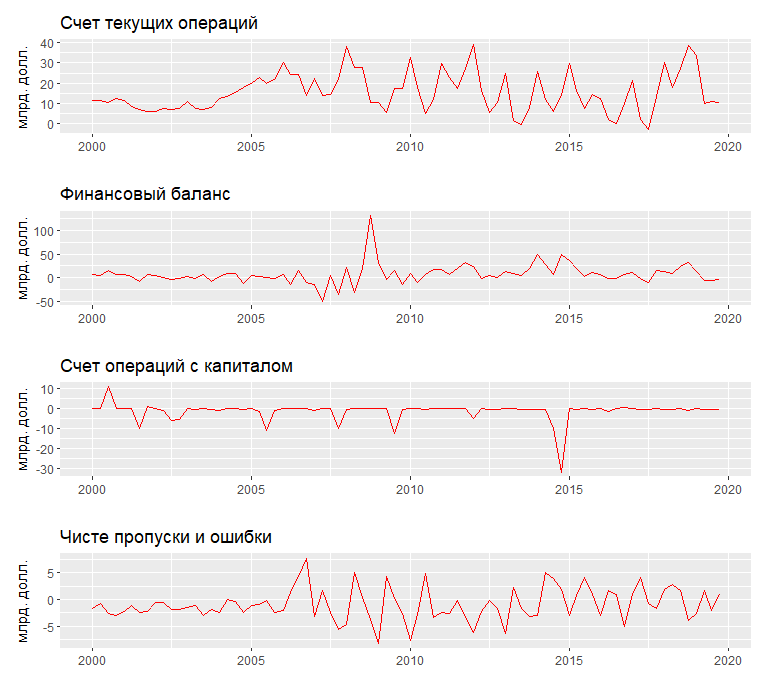
\includegraphics[width=\linewidth]{bal_str.png}
	\captionsetup{justification=centering,margin=0.5cm}
	\caption{Структура платежного баланса}\label{fi:structure_other}
\end{figure}


\begin{figure}[htp!]
	\centering
	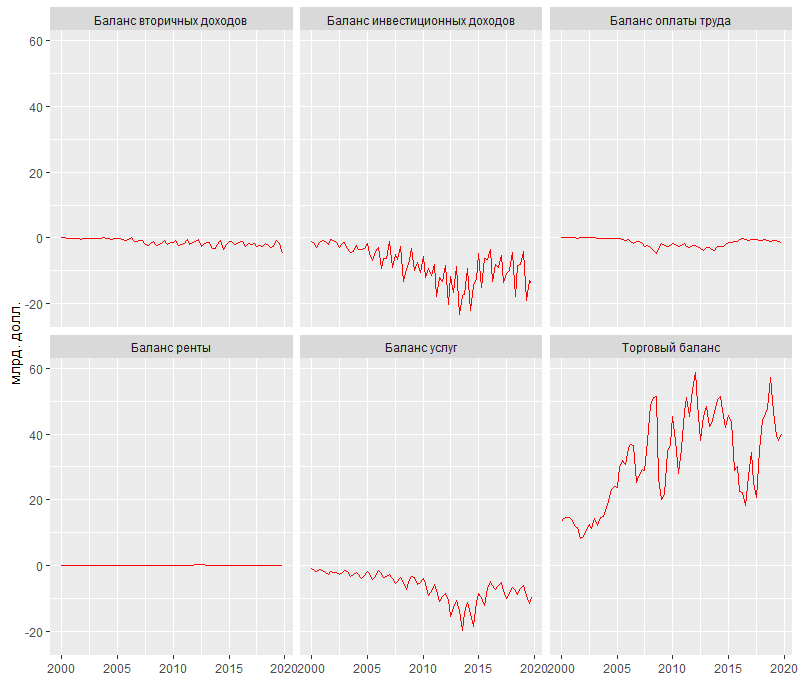
\includegraphics[width=\linewidth]{cur_acc_comp.png}
	\captionsetup{justification=centering,margin=0.5cm}
	\caption{Структура счета текущих операций}\label{fi:structure}
\end{figure}

\newpage
\begin{figure}[htp!]
	\centering
	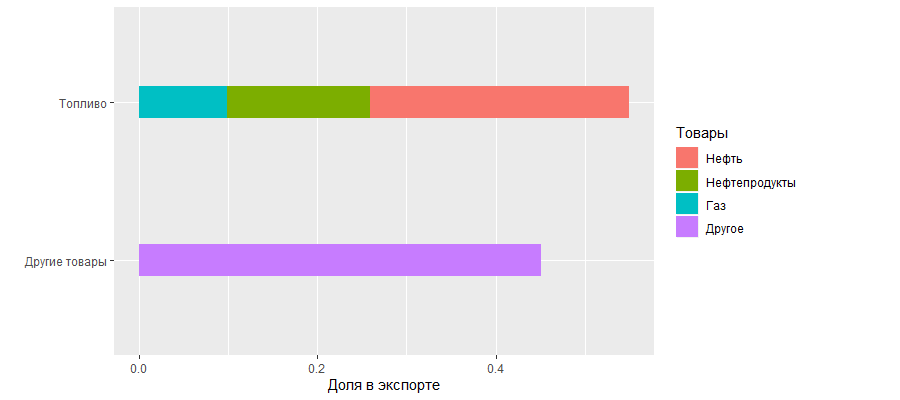
\includegraphics[width=18cm]{export_structure.png}
	\caption{Структура экспорта РФ, 2019 год}\label{fi:1}
	\captionsetup{justification=centering,margin=0.8cm}\label{fi:1}
	\caption*{\textit{Доля нефти, нефтепродуктов и газа в экспорте РФ в 2019 году составила $55\%$.}}
\end{figure}

\subsubsection{Уравнения}
Рассмотрим уравнения модели.
Все оценки коэффициентов получаются путем минимизации целевой функции специального вида, который подробнее будет описан в следующем разделе.
Корректировка на сезонность осуществляется путем включения в модель на месячных данных одиннадцати дамми-переменных.
Значимые события учтены в модели при помощи дополнительных дамми—переменных.
В модели используются переменная $\text{dum\_1114}_t$, равная единице с ноября $2014$ года, времени окончательного перехода к режиму плавающего валютного курса и отмены регулярных интервенций,  и переменная $\text{dum\_2012}_t$, равная единице с января $2012$ года по июль $2015$ года, на период после мирового экономического кризиса $2008-2012$ года.
Во всех уравнениях модели, если необходимо, темп прироста переменной обозначается как $\text{var\_ratio}_{t} = \frac{\text{var}_t -\text{var}_{t-1}}{\text{var}_{t-1}} = \Delta \text{var}_t / \text{var}_{t-1}$, где $\text{var}_{t}$ — любая переменная.
Коэффициенты каждого блока уравнений и каждой системы оцениваются независимо.

\subsubsection*{Модель валютного курса (RUB/USD)}

Валютный курс моделируется в несколько шагов. 
Из-за нестационарности ряда (см. рисунок \ref{fi:2}) в качестве объясняемой переменной в уравнении используется прирост валютного курса, а не абсолютное значение.

\vspace{2cm}

\begin{figure}[htp!]
	\centering
	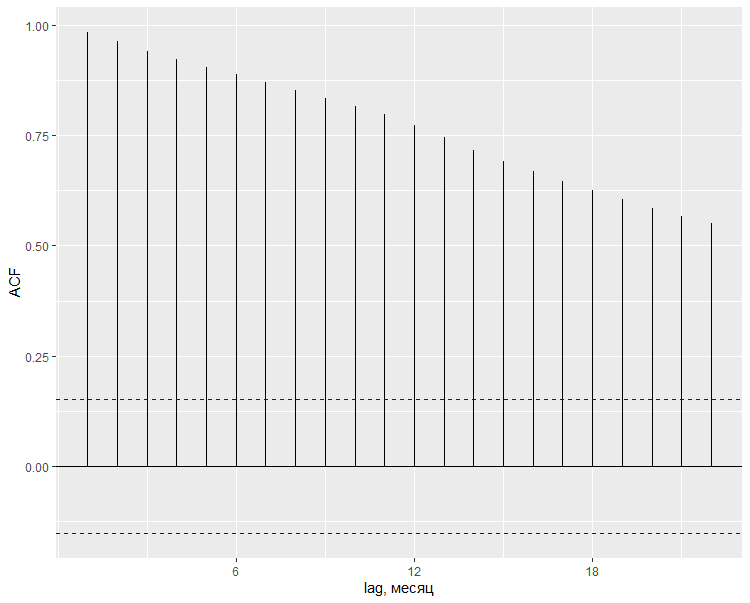
\includegraphics[width=14cm]{acf_rub_usd.png}
	\caption{Автокорреляционная функция для ряда валютного курса RUB/USD}\label{fi:2}
	\captionsetup{justification=centering,margin=0.5cm}
	\caption*{\textit{Значение статистики KPSS для проверки гипотезы о стационарности ряда, равно $2.9$, $p-value <0.01$. Гипотеза отвергается на любом разумном уровне значимости.}}
\end{figure}

\newpage
\begin{enumerate}[\begingroup\color{violet} 1.\endgroup]
	\item На первом шаге оценивается уравнение, где $\text{rub\_usd\_growth}_{t}$ — это прирост величины валютного курса по сравнению с предыдущим периодом (месяцем):
	\begin{align*}
\text{rub\_usd\_}&\text{growth}_{t} = c_1 + c_2 \cdot \text{rub\_usd\_growth}_{t-1} + c_3 \cdot \text{usd\_eur\_ratio}_{t} \\
& + \quad (c_4 + c_5 \cdot \text{dum\_1114}_t + c_6 \cdot \frac{\text{vcor}_t}{\text{usd\_rub}_{t-1}})\cdot \text{brent\_ratio}_t + \\
&  + \quad (c_7  + c_8 \cdot \text{dum\_1114}_t)\cdot \text{em\_index\_ratio}_t \\   
	& + \quad c_9 \cdot \text{dif\_r}_t \cdot \text{dum\_1114}_t + 
	\lsum_{i = 0, 1} c_{10+i}\cdot\text{r\_cur\_purch}_{t-i} + \varepsilon_{t}
	\end{align*}
	
	где $\text{dif\_r}_t$ — дифференциал процентных ставок, вычисляемый как разность между ключевой ставкой ЦБ РФ и доходностью 10-летних государственных облигаций США.

	\item На втором шаге на основании полученного прогноза прироста строится несколько прогнозов валютного курса с разной стартовой точкой с шагом в квартал (с июня 2006 г., с сентября 2006 г. и т.д.)
	\item На третьем шаге итоговый прогноз валютного курса получается путем усреднения в каждой точке прогнозов, полученных на втором шаге. 
	Гипотеза заключается в том, что усреднение прогнозов, построенных на разные горизонты, позволит уловить как краткосрочную, так и среднесрочную динамику валютного курса.
\end{enumerate}

\subsubsection*{Модель покупки валюты Минфином в рамках бюджетного правила}

Анализ динамики исполнения бюджетного правила также является важной частью модели внешнеэкономической деятельности РФ.
Согласно этому правилу устанавливается некоторая цена отсечения, выше которой все нефтегазовые сверходоходы поступают в Фонд национального благосостояния (ФНБ).
На данный момент базовой ценой отсечения являлась усредненная за $2017$ год цена барреля нефти, равная $40\$$ . 
Начиная с $2018$ года она индексируется на $2 \%$ в год.
Теоретически, валютное правило должно снижать зависимость экономики от резких колебаний на рынке энергоносителей, обеспечивая стабильность национальной валюты и покрытие дефицита бюджета при резком снижении доходов.

В модели покупка валюты по бюджетному правилу оценивается следующим уравнением:
\begin{align*}
\text{r\_cur\_}&\text{purch}_t = \text{r\_dum\_cur\_purch}_t \cdot (c_1 \cdot \text{r\_cur\_purch}_{t-1} + \\
& + \quad c_2 \cdot \text{r\_price\_cur\_purch}_t + \lsum_{i=0}^2 c_{i+3} \cdot \text{brent}_{t-i}) + \varepsilon_{t},
\end{align*}
где $\text{r\_dum\_cur\_purch}_t$ — дамми-переменная, равная единице в период $t$, когда Минфин выходил на валютный рынок.

\subsubsection*{Модели топливных рынков}
Модели топливных рынков представляют собой системы уравнений, в рамках которых моделируются три показателя: объем экспорта за соответствующий период, выручка от экспорта и средняя цена экспорта.
Каждая из систем оценивается независимо.
В работе предложены модели основных топливных ресурсов, экспортируемых из РФ: нефти, нефтепродуктов и газа.
\vspace{5mm}

\textit{Модель нефти:}
\begin{align*} 
\begin{cases}
\text{p\_exp\_oil}_t =&c_1 + \lsum_{i = 0}^{1}c_{2+i} \cdot \text{brent}_{t-i} + \varepsilon_{t,p}\\
\text{v\_exp\_oil}_t =&\lsum_{j = 1}^{11} d_j \cdot \text{dum}_t \cdot(a_1 + a_2 \cdot \text{v\_exp\_oil}_{t-3} + a_3 \cdot \text{usd\_rub}_{t-1} + \\ 
&+ \quad a_4 \cdot \text{p\_exp\_oil}_{t-3}) + \varepsilon_{t,v}\\
\text{r\_exp\_oil}_t =&\text{p\_exp\_oil}_t \cdot \text{v\_exp\_oil}_t + \varepsilon_{t,r}
\end{cases}
\end{align*}

\vspace{5mm}

\textit{Модель газа:}
\begin{align*} 
	\begin{cases}
		\text{p\_exp\_gas}_t =&c_1 + \text{dum\_2012}_t {+} \lsum_{i = 1,3,5,6}b_{i} \cdot \text{brent}_{t-i} + \lsum_{i = 3, 5} g_i \cdot \text{gas\_lng}_{t-i} + \\ 
		&+ \quad c_2 \cdot \text{gas\_europe}_t + \varepsilon_{t,p} \\
		\text{v\_exp\_gas}_t =&\lsum_{j = 1}^{11} d_j \cdot \text{dum}_t \cdot(a_1 + a_2 \cdot \text{v\_prod\_gas}_{t} + a_3 \cdot \text{usd\_eur}_{t} + \\ 
		&+ \quad a_4 \cdot \frac{\Delta\text{usd\_rub}_{t-1}}{\text{usd\_rub}_{t-2}} +
		\lsum_{i = 1, 7} p_i \cdot \widehat{ \text{p\_exp\_gas}}_{t-i})+  \varepsilon_{t,v}\\
		\text{r\_exp\_gas}_t =&\text{p\_exp\_gas}_t \cdot \text{v\_exp\_gas}_t + \varepsilon_{t,r}
	\end{cases}
\end{align*}

\vspace{5mm}

\textit{Модель нефтепродуктов:}
\begin{align*} 
	\begin{cases}
		\text{p\_exp\_op}_t =&c_1 + \lsum_{i = 0}^{3}c_{2 + i} \cdot \text{brent}_{t-i} + \varepsilon_{t,p} \\
		\text{v\_exp\_op}_t =&\lsum_{j = 1}^{11} d_j \cdot \text{dum}_t \cdot (a_1 + a_2 \cdot \text{v\_prod\_op}_{t-1} + a_3 \cdot \frac{\text{usd\_rub}_{t-1}}{\text{usd\_rub}_{t-2}} + \\  
		&+ \quad a_4 \cdot \widehat{ \text{p\_exp\_op}_{t-1}}) + \varepsilon_{t,v} \\
		\text{r\_exp\_op}_t =&\text{p\_exp\_op}_t \cdot \text{v\_exp\_op}_t + \varepsilon_{t,r}
	\end{cases}
\end{align*}


\subsubsection*{Модель платежного баланса}

Модель платежного баланса предназначена для прогнозирования основных компонент платежного баланса при заданных экзогенных переменных либо для восстановления отсутствующих исторических значений.
На уровне агрегатов в модели исследуется динамика счета текущих операций и финансового счета.
Счет операций с капиталом не моделируется, а при построении прогнозов его значение принимается равным нулю.
Это предположение вызвано динамикой платежного баланса за рассматриваемый период, в течение которого счет операций с капиталом, за исключением нескольких единичных случаев, приблизительно равнялся нулю.

\newpage
\begin{enumerate}[\begingroup\color{violet} 1.\endgroup]
	\item Счет текущих операций
	\begin{itemize}[label = \labelitemiii]
		\item Экспорт
		
		Совокупный экспорт товаров моделируется в два шага.
		Сначала оценивается система для совокупного экспорта товаров, который равен суммарной выручке от экспорта нефти, нефтепродуктов и газа и выручке от экспорта других товаров. 
		На этом шаге оценивается следующая система:
		\begin{align*}
		\begin{cases}        
		\text{r\_exp\_othg}_t =& \lsum_{j = 1}^{11} d_j \cdot \text{dum}_t \cdot (c_1 +
		(c_2 \cdot \widehat{\text{r\_exp\_fuels}}_t +  \\
		& + c_3 \cdot \text{dum\_1114}_t \cdot \widehat{\text{r\_exp\_fuels}}_t) + 
		\varepsilon_{t, othg} \\
		\text{r\_exp\_goods}_t =& \widehat{\text{r\_exp\_fuels}}_t + \widehat{\text{r\_exp\_othg}}_t + \varepsilon_{t, gds},
		\end{cases}
		\end{align*}
		где 
		\[
		 \widehat{\text{r\_exp\_othg}}_t =\widehat{\text{r\_exp\_oil}}_t + \widehat{\text{r\_exp\_op}}_t + \widehat{\text{r\_exp\_gas}}_t.
		\]
		
		На втором шаге моделируется экспорт услуг, а также вводятся уравнения на торговый баланс, по определению равный разности между экспортом и импортом товаров, и баланс услуг, равный разности между экспортом и импортом услуг
\begin{align*}	
		\begin{cases}        
			\text{r\_exp\_serv}_t =& \lsum_{j = 1}^{11} d_j \cdot \text{dum}_t \cdot (c_1 + c_2 \cdot \widehat{\text{r\_exp\_goods}}_t + \\ &
			+ \quad c_3 \cdot \widehat{\text{r\_imp\_serv}}_t) + \varepsilon_{t, srv}\\
			\text{r\_bal\_trade}_t =& \widehat{\text{r\_exp\_goods}}_t - \widehat{\text{r\_imp\_goods}}_t + \varepsilon_{t, bt}\\
			\text{r\_bal\_serv}_t =& \widehat{\text{r\_exp\_serv}}_t - \widehat{\text{r\_imp\_serv}}_t + \varepsilon_{t, bs}
		\end{cases}
	\end{align*}
		 
		\item Импорт
		
		Совокупный импорт моделируется при помощи одной системы, включающей отдельные уравнения на импорт товаров и услуг и балансовое соотношение на равенство совокупного импорта за период сумме импорта товаров и услуг:
		
		\begin{align*}
		\begin{cases}        
		\text{r\_imp\_goods}_t =& \lsum_{j = 1}^{11} d_j \cdot \text{dum}_t \cdot (c_1 +
		\frac{c_2\cdot\text{n\_c}_{t-1} +
			c_3\cdot\text{n\_j}_{t-1} +
				c_4\cdot\text{n\_ds}_{t-1}}{\text{usd\_rub}_{t-1}} + \\  
			& + \quad c_5 \cdot \widehat{\text{r\_exp\_goods}}_{t-1} + \varepsilon_{t, gds} \\
		\text{r\_imp\_serv}_t =& \lsum_{j = 1}^{11} \rho_j \cdot \text{dum}_t \cdot (a_1 +
		\frac{a_2 \cdot \text{n\_c}_{t-1} +
			a_3 \cdot \text{n\_j}_{t-1} +
			a_4  \cdot \text{n\_ds}_{t-1}}{\text{usd\_rub}_{t-1}} + \\  
		&+ \quad a_5 \cdot \widehat{\text{r\_imp\_goods}}_{t-1} + \varepsilon_{t, srv} \\
		\text{r\_imp\_all}_t =& \widehat{\text{r\_imp\_goods}}_t + \widehat{\text{r\_imp\_serv}}_t + \varepsilon_{t, all}
		\end{cases}
		\end{align*}
		
		Разность подходов к моделированию экспорта и импорта объясняется более сложной структурой экспорта услуг.
		Нередко в него попадают статистические расхождения и ошибки, связанные с записью импорта товаров, поэтому кажется логичным моделировать импорт товаров и услуг в одной системе.
		Экспорт услуг является более разнородным и моделируется отдельно, балансируя торговый баланс.
		\item Баланс оплаты труда
		
		Баланс оплаты труда показывает сальдо между заработными платами полученными гражданами РФ за границей и переведенными в РФ и заработными платами нерезидентов государства, переведенными зарубеж.
		Для России характерно отрицательные значения баланса оплаты труда.
		Он моделируется следующим уравнением
		
		\begin{align*}
			\text{r\_bal}\text{\_wage}_t =& \lsum_{j = 1}^{11} d_j \cdot \text{dum}_t \cdot (c_1 + 
			 c_2 \cdot \widehat{ \text{r\_exp\_oil}}_t + c_3 \cdot \widehat{ \text{r\_exp\_othg}}_t + \\
			 & + \quad c_4 \cdot \widehat{ \text{r\_exp\_serv}}_t + c_5 \cdot \widehat{ \text{r\_imp\_serv}}_t) + \varepsilon_{t, bw} 
		\end{align*}
		
		\item Баланс ренты и вторичных доходов
		
		Баланс ренты фиксирует доходы, получаемые резидентами РФ за предоставление в пользование природных ресурсов нерезидентам. 
		На протяжении всего рассматриваемого периода он принимает либо нулевые, либо очень маленькие положительные значения.
		Баланс вторичных доходов отражает перемещение трансфертов между резидентами и нерезидентами. 
		Как правило, в платежном балансе РФ этот счет принимает маленькие отрицательные значения.
		В рамках модели изучается динамика суммарного показателя баланса ренты и баланса вторичных доходов.
		Она описывается следующим уравнением:
		\begin{align*}
		\text{r\_rent\_sinc}_t = & \lsum_{j = 1}^{11} d_j \cdot \text{dum}_t \cdot (c_1 + c_2 \cdot \widehat{ \text{r\_exp\_goods}}_t + \\
		& c_3 \cdot \widehat{ \text{r\_exp\_serv}}_t) + \varepsilon_{t, rs} 
		\end{align*} 
		
		\item Баланс инвестиционных доходов
				
		Баланс инвестиционных доходов отражает выплаты по ценным бумагам и другие выплаты, связанные с различными формами собственности.
		В этой модели баланс инвестиционных доходов балансирует счет текущих операций и оценивается с ним в одной системе.
		
		\begin{align*}
		\begin{cases}
		\text{r\_bal\_inv}_t =& \lsum_{j = 1}^{11} d_j \cdot \text{dum}_t \cdot (c_1 + c_2 \cdot \widehat{\text{r\_bal\_trade}}_t + \\
		& + \quad c_3 \cdot \widehat{\text{r\_bal\_serv}}_t) + \varepsilon_{t, bi} \\ 
		\text{r\_cur\_acc}_t =& \widehat{\text{r\_bal\_inv}}_t + \widehat{ \text{r\_bal\_rent\_sinc}}_t + \widehat{\text{r\_bal\_wage}}_t +\\ & + \quad \widehat{\text{r\_bal\_serv}}_t +
		\widehat{\text{r\_bal\_trade}}_t + \varepsilon_{t, ca} 
		\end{cases}
		\end{align*} 
	\end{itemize}
		\item  Изменение резервных активов
		
		Резервные активы являются частью финансового счета.
		Они включают в себя высоколиквидные иностранные активы, контролируемые Правительством и ЦБ и используются в основном для проведения интервенций на валютном рынке.
		В силу смены режима монетарной политики в России, динамика счета моделируется двумя различными уравнениями.
		Первое уравнение предназначено для восстановления динамики счета до $2015$ года, то есть до окончательного введения режима инфляционного таргетирования, и учитывает в качестве фактора ширину валютного коридора $\text{vcor}_t$.
		Для восстановления динамики после $2015$ года и получения прогнозов используется второе уравнение, учитывающее покупку валюты Минфином в рамках бюджетного правила.
		Для расчета коэффициентов уравнения оцениваются в системе.
		
		\begin{align*}
		\begin{cases}
		\text{dif\_reserves}_t &= c_1 + c_2 \cdot \widehat{\text{dif\_reserves}}_{t-1} + \lsum_{j = 1}^{11} d_j \cdot \text{dum}_t + \\
		& + \quad c_3 \cdot \widehat{\text{r\_cur\_acc}}_{t} + c_4 \cdot \widehat{\text{r\_cur\_acc}}_{t-1} + \\
		& + \quad (c_5 + c_6 \cdot \frac{\text{vcor}_t}{\text{usd\_rub}_{t-1}}) \cdot \Delta \text{brent}_t + \\
		&+ \quad c_7 \cdot \Delta \text{usd\_rub\_}_t + c_8 \cdot \Delta \text{usd\_rub}_{t-1} + c_9 \cdot \Delta \text{usd\_eur}_{t}+ \varepsilon_{t, df_{1}}\\ 
		\text{dif\_reserves2}_t &= a_1 + a_2 \cdot \widehat{\text{dif\_reserves}}_{t-1} + \lsum_{j = 1}^{11} f_j \cdot \text{dum}_t + \\
		&+ \quad a_3 \cdot \widehat{\text{r\_cur\_acc}}_{t} + a_4 \cdot \widehat{\text{r\_cur\_acc}}_{t-1} + a_5 \cdot \Delta \text{brent}_t + \\
		&+ \quad a_6 \cdot \Delta \text{usd\_rub\_}_t + a_7 \cdot \Delta \text{usd\_rub\_}_{t-1} + a_8 \cdot \Delta \text{usd\_eur}_А{t} + \\
		&+ \quad a_9 \cdot \widehat{\text{r\_cur\_purch}}_t +  a_{10} \cdot \widehat{\text{r\_cur\_purch}}_{t-1} + \varepsilon_{t, df_{2}} \\ 
		\end{cases}
		\end{align*}		
		\item Финансовый баланс
		
		Прогноз финансового баланса получается исходя из его определения в платежном балансе, как разницы между суммой счета текущих операций, операций с капиталом и чистых пропусков и ошибок и изменением резервных активов:
		\[
		\widehat{\text{r\_bal\_fin}}_t = \widehat{\text{r\_cur\_acc}}_t +\widehat{\text{r\_cap\_acc}}_t + \widehat{\text{r\_errors}}_t - \widehat{\text{dif\_res}}_t
		\]
		
		\newpage
		\item Чистые ошибки и пропуски
		
		Счет чистых ошибок и пропусков моделируется с помощью дамми-переменых, так как имеет ярко выраженную сезонную структуру.
		
		\begin{align*}
		\text{r\_errors}_t = c_1 + c_2\cdot \Delta \text{brent}_t  + \lsum_{j = 1}^{11} d_j \cdot \text{dum}_t
		\end{align*}
\end{enumerate}

\subsubsection{Целевая функция}\label{sub:costfunction}

Как было отмечено в разделе \hyperref[sub:data]{Данные}, месячные данные по многим переменным платежного баланса отсутствуют за длинные временные интервалы.
Тем не менее, для построения прогнозов в месячной разбивке хотелось бы учесть всю имеющуюся информацию, которая может содержаться также и в квартальных данных. 
Для таких целей нередко прибегают к использованию различных способов регуляризации.
В данной работе была введена целевая функция $E(.)$ особого вида, которая представляет собой квадратный корень из суммы ошибок прогноза на месячных данных с регуляризацией на ошибку квартального прогноза:
\[
E(y_m, \hat y_m, y_q, \hat y_q; \alpha) = || y_m - \hat y_m ||_2 + \alpha|| y_q - \hat y_q ||_2,
\]

где $y_m$ — фактические месячные значения временного ряда, $\hat y_m$ — восстановленные моделью значения этого ряда, $y_q$ — фактические квартальные значения, $\hat y_q$ — восстановленные квартальные значения, $\alpha$ — параметр регуляризации.

Функционал такого вида позволяет уловить одновременно краткосрочную динамику переменных, проявляющуюся на данных с более высокой частотностью, и среднесрочную динамику, которая может быть заметна только на квартальных данных.
Параметр регуляризации $\alpha$ может подбираться для каждого ряда отдельно путем простого перебора с некоторым шагом. 
Он показывает относительный вес ошибки прогноза на квартальных данных в целевом функционале, а именно, насколько сильно мы хотим учесть среднесрочную динамику при построении месячного прогноза.
Отметим, что подбор гиперпараметров — это отдельный исследовательский вопрос, и в этой работе для простоты  $\alpha$ принимается равной $1$ для всех восстанавливаемых рядов, то есть ошибки на месячных данных и на квартальных имеют равный вес.

Если оценивается не одно независимое уравнение, а целая система, то минимизируется суммарная ошибка по всем уравнениям в системе.

Восстановленное значение $\hat y_m$ месячных рядов получается путем подстановки коэффициентов в уравнение для данной переменной.
Восстановленное значение $\hat y_q$ квартальных рядов, получается простым суммированием прогнозов месячных значений за соответствующий квартал.

\subsection{Результаты модели}

На рисунках \ref{fi:3} - \ref{fi:6} представлены результаты работы четырех блоков модели. 
Оптимизация коэффициентов осуществлялась на данных с $2006$ по $2019$ гг. — последних актуальных месячных и квартальных данных по платежному балансу на момент написания работы.

В качестве моделей для сравнения были выбраны ARIMA, ets и сезонный наивный прогноз.
Параметры моделей ARIMA и ets подбирались автоматически по значению информационного критерия. 
В сезонной наивной модели прогноз для текущего месяца строился как значение ряда в тот же месяц в прошлом году.

В качестве метрик для сравнения качества прогнозов разными методами были выбраны метрики MAPE (mean absolute percentage error) и MASE (mean absolute scaled error).

\newpage 

\begin{figure}[htp!]
\centering
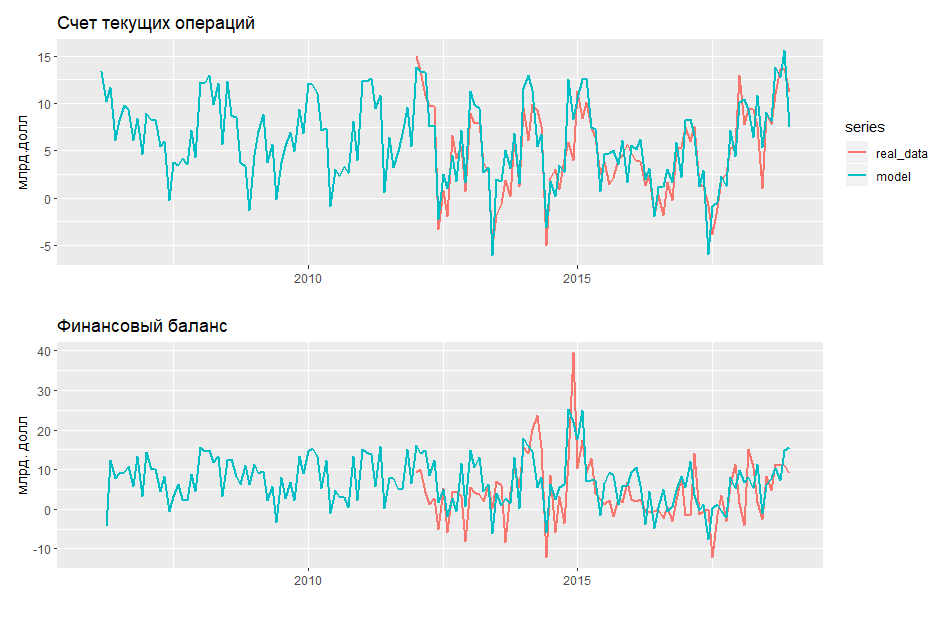
\includegraphics[width=19cm]{cur_fin.png}
\captionsetup{justification=centering,margin=0.5cm}
\caption{Модель платежного баланса: счет текущих операций и финансовый баланс}\label{fi:3}
\captionsetup{margin=0cm}
\caption*{\textit{На рисунках \ref{fi:3} и \ref{fi:4} представлены фактические и восстановленные значения основных агрегатов платежного баланса. 
Официальная статистика по платежному балансу в месячной разбивке доступна с $2012$ года.}}
\end{figure}

\begin{figure}[htp!]
	\centering
	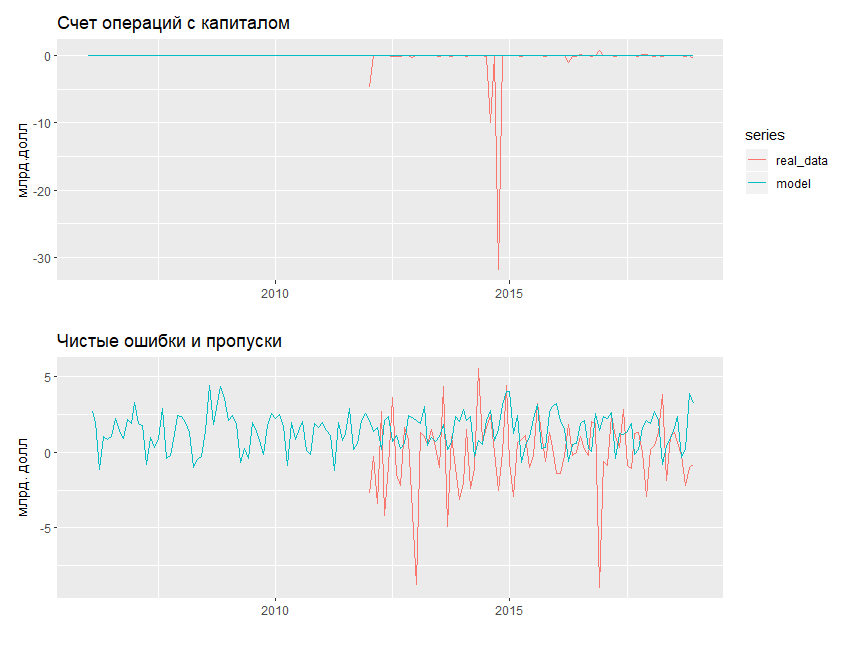
\includegraphics[width=19cm]{cap_er.png}
	\captionsetup{justification=centering,margin=0.5cm}
	\caption{Модель платежного баланса: счет операций с капиталом и чистые ошибки и пропуски}\label{fi:4}
\end{figure}

\newpage
\begin{figure}[htp!]
	\centering
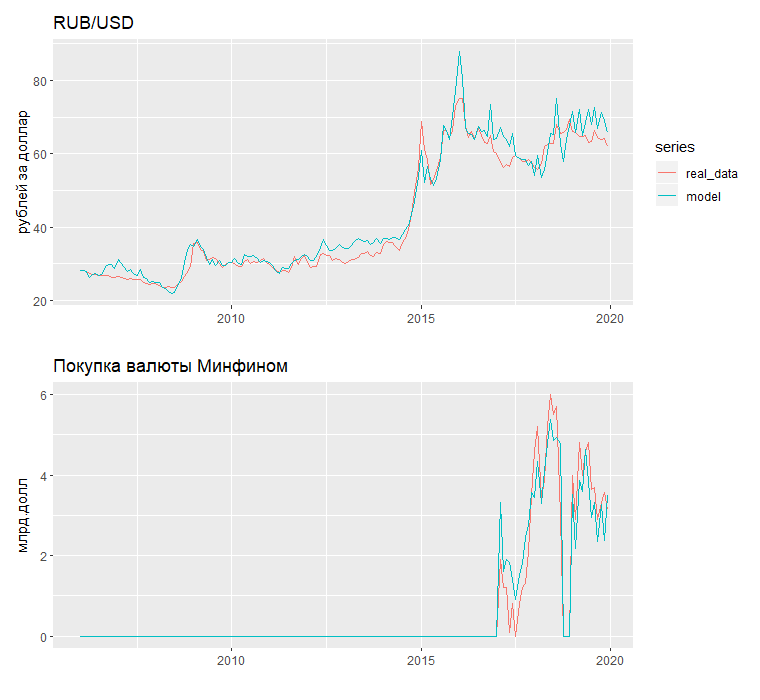
\includegraphics[width=19cm]{rub_purch.png}
\caption{Модели обменного курса и покупки валюты}\label{fi:5}
\captionsetup{justification = centering, margin=0cm}
\caption*{\textit{Верхняя панель: внутривыборочный прогноз для модели обменного курса RUB/USD;	
		нижняя панель: внутривыборочный прогноз для модели покупки валюты Минфином в рамках бюджетного правила.}}
\end{figure}

\newpage

\begin{figure}[htp!]
	\centering
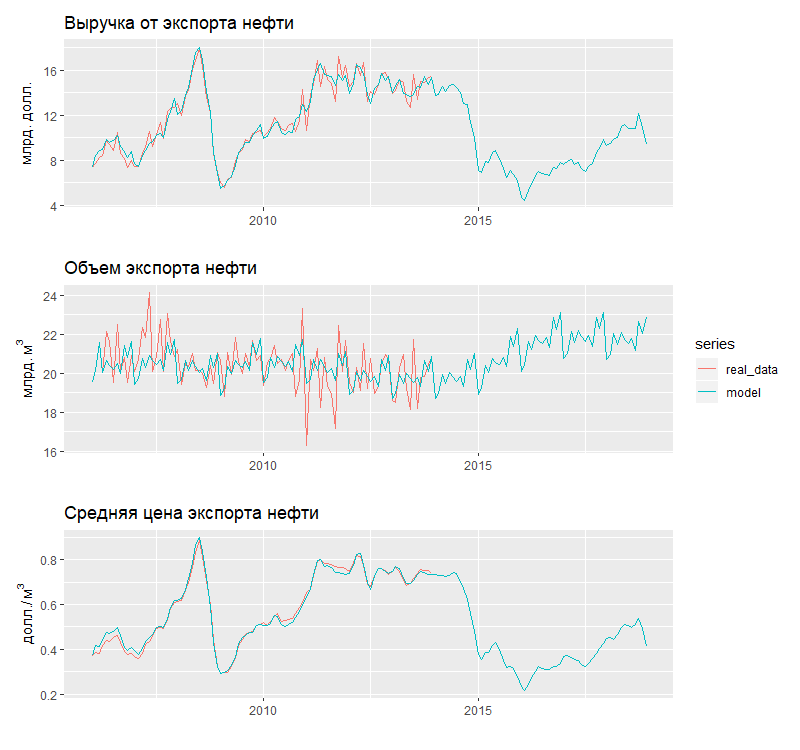
\includegraphics[width=\linewidth]{oil_model.png}
\caption{Модель экспорта нефти}\label{fi:5}
	\captionsetup{justification=centering,margin=0cm}
\caption*{\textit{На графике представлены фактические и восстановленные значения объемов и выручки от экспорта нефти. 
Средняя цена равна отношению выручки к объему.
Официальная статистика по экспорту топливных ресурсов в месячной разбивке доступна до $2013$ года.}}
\end{figure}


\begin{figure}[htp!]
	\centering
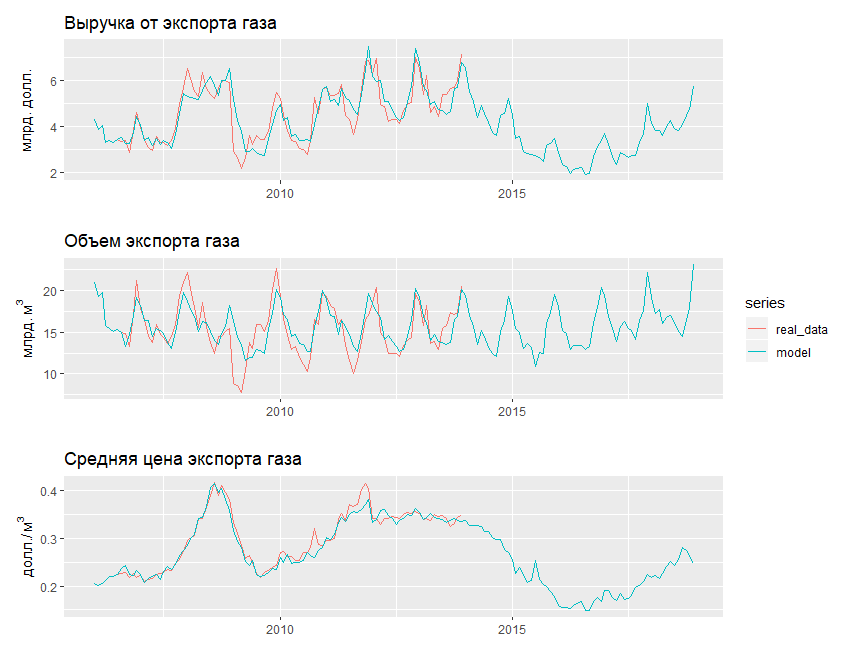
\includegraphics[width=19cm]{gas_model.png}
\caption{Модель экспорта газа}\label{fi:6}
\end{figure}



\begin{figure}[htp!]
	\centering
	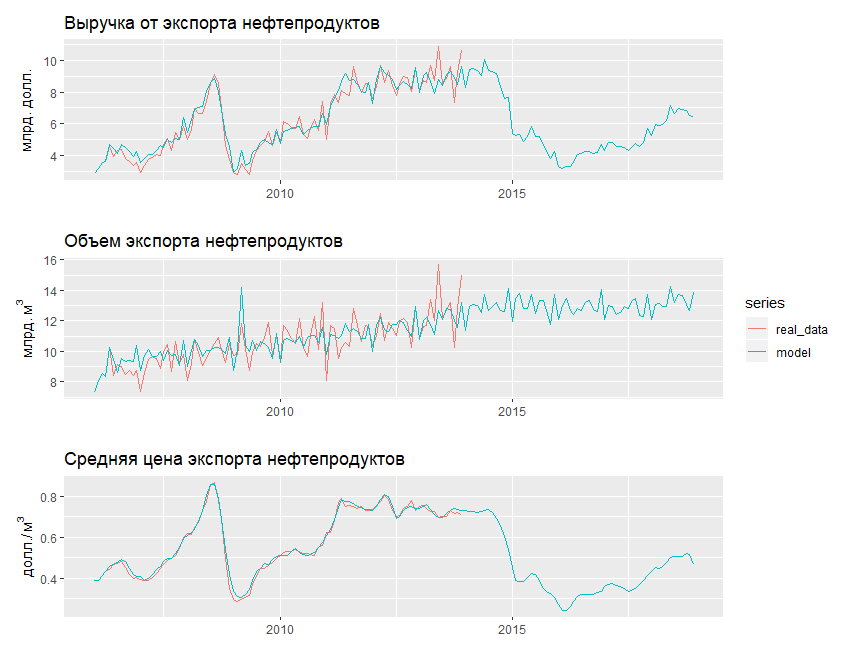
\includegraphics[width=19cm]{op_model.png}
	\caption{Модель экспорта нефтепродуктов}\label{fi:op_model}
\end{figure}

\newpage 

MAPE часто используется при оценке качества прогнозов в силу своей простоты и интерпретируемости, однако неустойчива к наличию нулей в ряду фактических данных. 

MAPE рассчитывается по формуле:
\[
MAPE = \frac{1}{n}\lsum_{t=1}^{n}\left|\frac{Y_t - \hat Y_t}{Y_t}\right|,
\]
где $Y_t$ — фактические значения ряда, $\hat Y_t$ — прогноз, $n$ — длина прогноза.

Метрика MASE имеет предсказуемое поведение при $Y_t \to 0$, что характерно для некоторых переменных платежного баланса, инвариантна к масштабу данных.
MASE рассчитывается по формуле:
\[
MASE = \frac{\frac{1}{J} \lsum_j |e_j|}{\frac{1}{T-1} \lsum_{t=2}^T|Y_t - Y_{t-1}|},
\]

где $J$ длина тестовой выборки, $T$ — длина обучающей выборки, $e_t$ — ошибка прогноза исследуемой модели, $Y_1, \ldots Y_T$ — значения целевой переменной в обучающей выборке. 
MASE можно интерпретировать как средний модуль ошибки изучаемой модели к среднему модулю ошибки наивного прогноза.
Значение MASE больше единицы говорит о том, что наивный прогноз более точный, чем прогноз рассматриваемой модели.

Для сравнения моделей исходная выборка была поделена на две части: обучающая выборка — до $2018$ года, тестовая выборка — $2019$ год.
Значение метрик для всех моделей и переменных представлено в таблице \ref{tab:4}.
Наименьшее значение метрики, соответствущее лучшей модели для данной переменной, выделено жирным цветом.
Из таблицы видно, что прогнозная сила модели внешнеэкономической деятельности оказалось выше для $18$ переменных из $27$ по MAPE и для $12$ переменных из $27$ по MASE (c MASE меньше $1$).

Стоит отметить, что большим преимуществом данной модели по сравнению с другими более простыми моделями временных рядов является возможность учета взаимосвязей между экзогенными и эндогенными переменными, имеющими отношение к внешнеэкономической деятельности РФ.
Модель является очень гибкой в плане подбора регрессоров, а уравнения могут быть легко модифицированы, например, с учетом изменений принципов монетарной политики, как это было сделано с уравнением на изменение резервов.


\newpage
\thispagestyle{empty}

\begin{center}
	\small
	\begin{tabular}{l|rr|rr|rr|rr}
		\toprule
		\multirow{2}{*}{series}&\multicolumn{2}{c|}{\textbf{bp\_model}}&\multicolumn{2}{c|}{\textbf{arima}}&\multicolumn{2}{c|}{\textbf{ets}}&\multicolumn{2}{c}{\textbf{snaive}}\\
		
		&MAPE & MASE & MAPE & MASE & MAPE & MASE & MAPE & MASE \\ 
		\midrule
		p\_exp\_gas & \textbf{0.02} & 1.93 & 0.05 & 2.22 & 0.06 & 2.37 & 0.03 & \textbf{1.16} \\ 
		p\_exp\_oil & \textbf{0.01} & \textbf{0.43} & 0.04 & 1.54 & 0.04 & 1.63 & 0.04 & 1.72 \\ 
		p\_exp\_op & \textbf{0.02} & \textbf{0.91} & 0.08 & 5.07 & \textbf{0.02} & 1.52 & 0.04 & 2.54 \\ 
		r\_bal\_fin & \textbf{1.61} & \textbf{0.96} & 2.73 & 1.07 & 4.35 & 1.39 & 3.37 & 1.63 \\ 
		r\_bal\_inv & 0.36 & 1.09 & \textbf{0.28} & \textbf{0.52} & 0.29 & 0.56 & 0.33 & 0.63 \\ 
		r\_bal\_rent\_sinc & \textbf{0.44} & 2.02 & 0.55 & 0.77 & 0.58 & 0.84 & 0.49 & \textbf{0.73} \\ 
		r\_bal\_serv & 2.14 & 1.21 & 0.26 & 1.26 & \textbf{0.13} & 0.62 & 0.22 & \textbf{1.06} \\ 
		r\_bal\_trade & 0.17 & 1.72 & \textbf{0.14} & \textbf{1.31} & 0.35 & 3.26 & 0.25 & 2.39 \\ 
		r\_bal\_wage & 0.25 & \textbf{1.53} & 0.33 & 4.35 & 0.35 & 5.04 & \textbf{0.17} & 3.21 \\ 
		r\_cur\_account & \textbf{0.36} & \textbf{1.63} & 5.83 & 2.86 & 4.36 & 2.31 & 2.49 & 1.84 \\ 
		r\_cur\_purch & \textbf{0.20} & \textbf{0.59} & 1.13 & 6.03 & 1.00 & 5.43 & 0.48 & 2.41 \\ 
		r\_dif\_reserves & 1.28 & \textbf{1.11} & 0.82 & 1.48 & \textbf{0.59} & 1.16 & 1.19 & 1.68 \\ 
		r\_errors & 1.90 & 0.95 & 1.11 & 0.67 & \textbf{1.03} & \textbf{0.61} & 1.86 & 0.88 \\ 
		r\_exp\_all & \textbf{0.05} & \textbf{0.90} & 0.08 & 1.53 & 0.06 & 1.09 & 0.07 & 1.40 \\ 
		r\_exp\_gas & \textbf{0.08} & 0.88 & 0.12 & 1.05 & 0.09 & \textbf{0.73} & 0.14 & 1.22 \\ 
		r\_exp\_goods & \textbf{0.03} & \textbf{0.54} & 0.09 & 1.69 & 0.07 & 1.40 & 0.08 & 1.53 \\ 
		r\_exp\_oil &\textbf{0.04} & 0.90 & 0.07 & \textbf{0.87} & 0.07 & 0.90 & 0.07 & 0.91 \\ 
		r\_exp\_op & \textbf{0.08} & 0.87 & 0.09 & \textbf{0.65} & 0.12 & 0.81 & 0.11 & 0.79 \\ 
		r\_exp\_othg & 0.05 & \textbf{0.49} & 0.05 & 0.79 & \textbf{0.04} & 0.70 & 0.06 & 0.91 \\ 
		r\_exp\_serv & 0.19 & 1.16 & 0.05 & \textbf{0.47} & \textbf{0.04} & 0.42 & 0.06 & 0.60 \\ 
		r\_imp\_all & \textbf{0.04} & \textbf{0.35} & 0.07 & 1.02 & 0.07 & 0.99 & 0.05 & 0.77 \\ 
		r\_imp\_goods & \textbf{0.04} & \textbf{0.37} & 0.06 & 0.88 & 0.09 & 1.29 & 0.05 & 0.81 \\ 
		r\_imp\_serv & 0.16 & 1.31 & 0.08 & 0.82 & \textbf{0.04} & \textbf{0.34} & 0.06 & 0.61 \\ 
		rub\_usd & \textbf{0.06} & \textbf{1.61} & 0.11 & 6.37 & 0.13 & 7.75 & \textbf{0.06} & 3.63 \\ 
		v\_exp\_gas & \textbf{0.08} & \textbf{0.84} & 0.14 & 1.36 & 0.09 & 0.92 & 0.14 & 1.36 \\ 
		v\_exp\_oil & \textbf{0.04} & 1.09 & 0.05 & 0.74 & 0.05 & \textbf{0.72} & \textbf{0.04} & 0.61 \\ 
		v\_exp\_op & \textbf{0.08} & 0.95 & 0.10 & \textbf{0.74} & 0.10 & 0.76 & 0.11 & 0.84 \\ 
		aq\_assets & \textbf{0.08} & 0.95 & 0.10 & \textbf{0.74} & 0.10 & 0.76 & 0.11 & 0.84 \\ 
		aq\_obl & \textbf{0.08} & 0.95 & 0.10 & \textbf{0.74} & 0.10 & 0.76 & 0.11 & 0.84 \\ 
		\bottomrule
	\end{tabular}
\captionsetup{justification=centering,margin=2cm}
\captionof{table}{Метрики качества для модели внешнеэкономической деятельности и бенчмарков}\label{tab:4}
\end{center}
\newpage
\subsection{Сценарные прогнозы}
Одним из значимых преимуществ модели платежного баланса РФ, описанной в этой работе, является возможность строить прогнозы эндогенных переменных при разных сценариях и изучать устойчивость платежного баланса в ответ на различные внешние шоки.
Под сценарием понимается некоторая заданная либо спрогнозированная траектория экзогенных переменных. 
Устойчивостью платежного баланса в этой работе мы будем называть сохранение положительного сальдо счета текущих операций в ответ на шоки экзогенных переменных.

В этой работе представлены сценарные прогнозы на $2020$ год.
Проверить работоспособность модели именно на этом временном промежутке кажется особенно интересным, так как в $2020$ году экономика России оказалась в кризисной ситуации, вызванной одновременно пандемией коронавируса и изменением конъюнктуры топливных рынков, резким падением цен на нефть и ослаблением курса рубля.

Так как ситуация, сложившаяся в мировой экономике вообще и в российской, в частности, является беспрецедентной, высока неопределенность относительно дальнейшего развития событий.
Пока что строить долгосрочные прогнозы может быть затруднительно, однако кажется разумным рассмотреть несколько сценариев «кризисного» развития экономики на ближайший, $2020$, год.
Логично ожидать снижение различных показателей внешнеэкономической деятельности, хотя бы в первых двух кварталах.
Кроме того, уже в марте $2020$ года цена на нефть опустилась ниже цены отсечения, предусмотренной бюджетным правилом, чего со времени перехода к режиму плавающего валютного курса не наблюдалось.
Отсюда разумно ожидать от Минфина продажи валюты для компенсации выпадающих доходов.
Понятно, что простые модели временных рядов, рассмотренные в предыдущем разделе, не способны уловить такие резкие изменения динамики переменных и, кроме того, предоставить несколько возможных траекторий прогнозируемых рядов

Для начала введем базовый сценарий.
В качестве ориентиров будем использовать базовый сценарий ЦБ \cite{cbr2020}, опубликованный после заседания Банка России от $24$ апреля $2020$ года, а также  аналитические материалы сайта Банки.ру.
В качестве оптимистичного сценария будем опираться на прогнозы Минэконом Развития «Сценарные условия прогноза социально-экономического
развития на 2019–2024 годы» \cite{minec2019}, которые были опубликованы в апреле $2019$ года, и, как минимум, не учитывали последствия кризиса из-за пандемии коронавируса.
Пессимистичным прогнозом будем считать отклонение экзогенных переменных от базового сценария на $5-10 \%$  в зависимости от типа переменной.
Экзогенные переменные, по которым на момент написания работы не было официального прогноза на $2020$ год, предсказаны сезонной наивной моделью, то есть по таким переменным для каждого месяца (квартала) $2020$ года в качестве прогноза было использовано значение соответствующего месяца (квартала) $2019$ года. 
Подробнее предположения изложены в таблице \ref{tab:5}.  
В таблице представлены средние значения показателя за $2020$ год, если не указано иное.

\begin{center}
	\small
		\begin{tabular}{c| c | c | c}
		Переменная & Базовый & Оптимистичный & Пессимистичный \\
		\toprule
		 Brent & $33$ & $ 64.9$ & $27$ \\
		$\Delta$ ВВП &  $-5.5 \%$  & $0\%$ &  $-8\%$  \\
		Ключевая ставка &  $5.5 \%$ до $07.20$,  & $5.5 \%$ до $07.20$, &  $5.5 \%$\\
		&$5 \%$ до $12.20$ & $5 \%$ до $10.20$, $4.5 \%$ до $12.20$ & \\
		USD/EUR & $1.1$ & $1.2$ & $1.08$ \\
		Цена отсечения & $42.44$ & $42.44$ & $42.44$\\
		\bottomrule
	\end{tabular}
	\captionof{table}{Сценарии экзогенных переменных}\label{tab:5}
	\normalsize
\end{center}

На рисунках \ref{fi:7}-\ref{fi:9} представлены полученные траектории некоторых эндогенных переменных модели при разных сценариях.

\begin{figure}[htp]
	\centering
	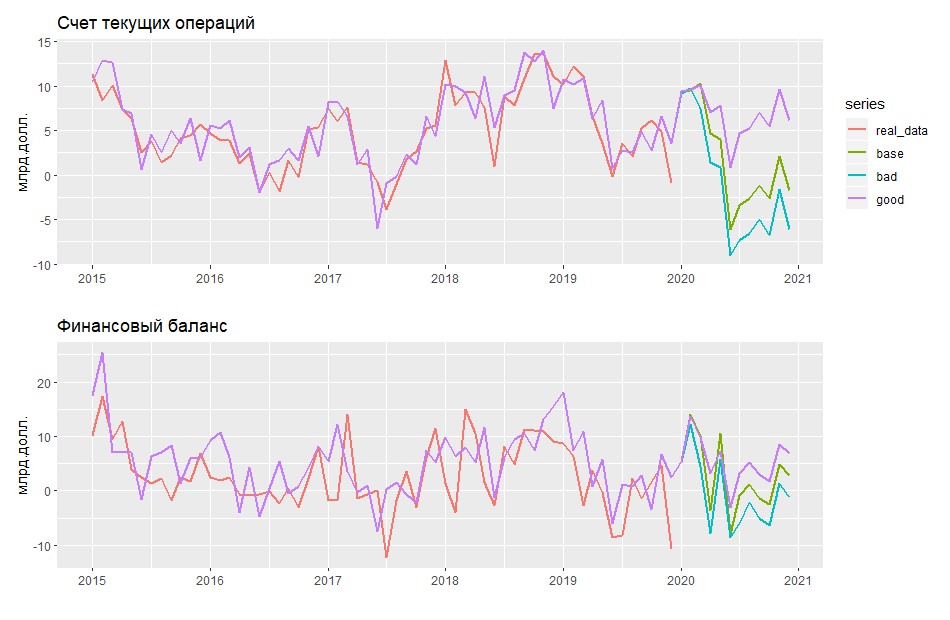
\includegraphics[width=18cm]{cur_2015.png}
	\caption{Компоненты платежного баланса}\label{fi:7}
\end{figure}

\begin{figure}[htp]
	\centering
	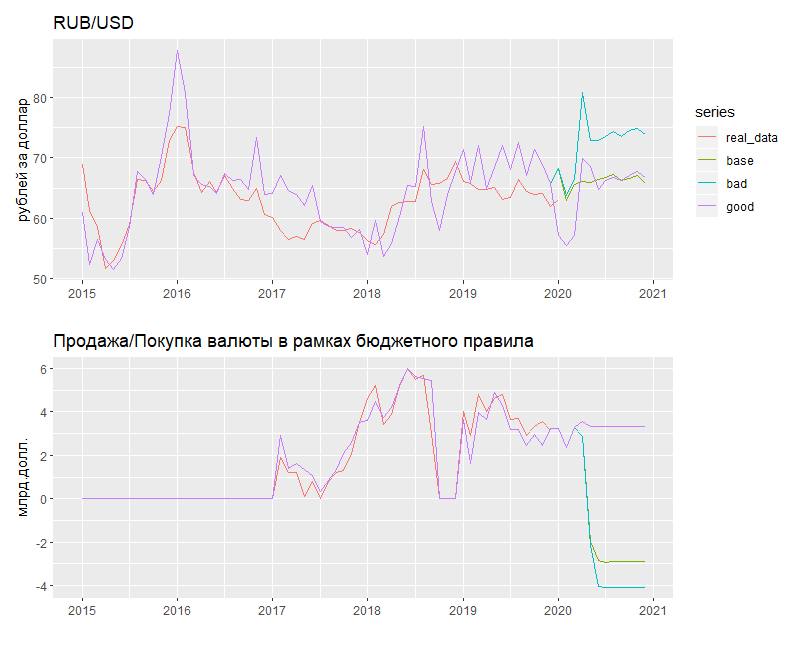
\includegraphics[width=18cm]{rub_2015.png}
	\caption{Валютный курс и покупка валюты Минфином}\label{fi:8}
\end{figure}

\begin{figure}[htp]
	\centering
	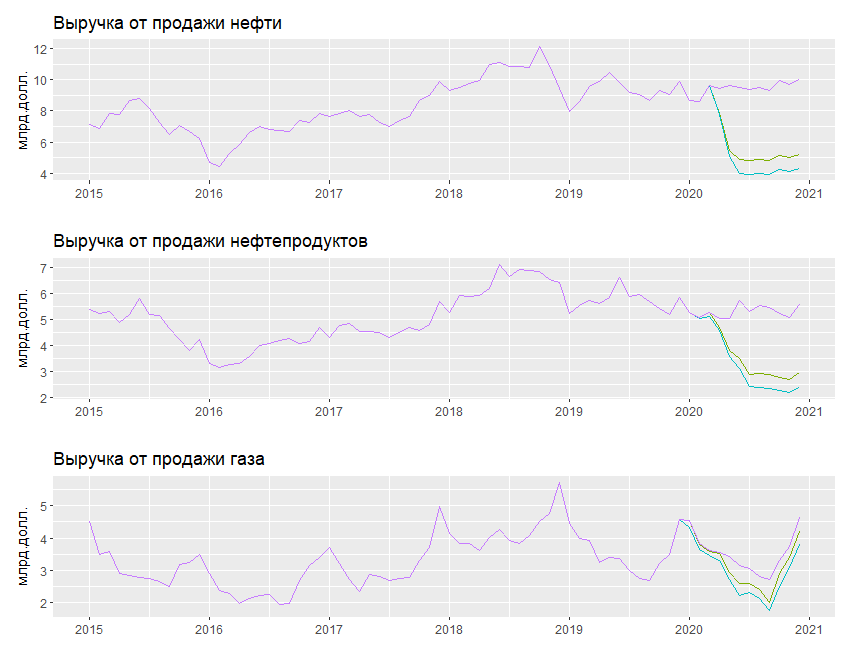
\includegraphics[width=18cm]{fuels_2015.png}
	\caption{Выручка от экспорта топливных ресурсов}\label{fi:9}
\end{figure}

\newpage

На графиках видно, что в базовом и пессимистичном сценариях на протяжении $2020$ года ожидается дефицит счета текущих операций.
Основным драйвером дефицита является резкое падение сальдо торгового баланса, вызванное в свою очередь падением выручки от экспорта нефти и ослаблением курса рубля к доллару.
Кроме того, базовый и пессимистичный сценарии предполагают продажу валюты Минфином, что соответствует логике бюджетного правила, согласно которой Центральный Банк продает накопленную валюту для компенсации потерь при цене нефти ниже цены отсечения.

В оптимистичном сценарии основные переменные, характеризующие внешнеэкономическую деятельность, повторяют траекторию прошлого года с некоторым снижением. 
При этом сохраняется положительное сальдо счета текущих операций, а Минфин продолжает покупку валюты в рамках бюджетного правила.

\newpage
\section{Заключение}

В данной работе предложена модель внешнеэкономической деятельности РФ, включающая блок платежного баланса в разбивке на отдельные счета и их компоненты, уравнение валютного курса (RUB/USD), уравнение покупки валюты в рамках бюджетного правила и блок моделей топливных ресурсов (нефти, нефтепродуктов и газа).
Модель показала лучшую прогнозную силу по сравнению с более простыми моделями временных рядов для большинства рассмотренных переменных.


Значимым преимуществом модели является возможность построения сценарных прогнозов.
В работе представлены сценарные прогнозы на $2020$ год для трех сценариев (базового, оптимистичного, пессимистичного), предполагающих различные уровни цен на нефть, темп падения ВВП, ключевую ставку.
Полученные прогнозы показывают высокую зависимость устойчивости (способности поддерживать профицит счета текущих операций) платежного баланса РФ от цен на нефть.
В базовом и пессимистичном сценариях, при среднем уровне цен на нефть марки Brent ниже цены отсечения, на протяжении $2020$ года ожидается дефицит счета текущих операций.


\newpage

\printbibliography

\end{document}